\documentclass[11pt,a4paper]{article}
\usepackage[margin=2.5cm]{geometry}
\usepackage[utf8]{inputenc}
\usepackage[T1]{fontenc}
\usepackage{amsmath,amssymb,physics}
\usepackage{booktabs}
\usepackage{float}
\usepackage{graphicx}
\usepackage{hyperref}
\usepackage{enumitem}
\usepackage{caption}
\usepackage{tcolorbox}
\tcbuselibrary{skins,breakable}

\newtcolorbox{resultbox}[1][]{enhanced,breakable,
  colback=blue!4!white,colframe=blue!40!black,
  fonttitle=\bfseries,title={#1},boxrule=0.6pt,arc=4pt}
\newtcolorbox{gapbox}[1][]{enhanced,breakable,
  colback=orange!6!white,colframe=orange!60!black,
  fonttitle=\bfseries,title={#1},boxrule=0.6pt,arc=4pt}

\hypersetup{colorlinks=true,linkcolor=blue,citecolor=blue,urlcolor=blue}

\title{\textbf{Saturated Superfluid Vacuum~VI-b}\\[0.4em]
\large Galactic Morphology as Overtone Structure}
\author{Stig Norland\\
\small Independent Researcher, Bergen, Norway}
\date{Draft}

\begin{document}
\maketitle

\begin{abstract}
This paper is the morphology companion to Paper~VI-a~\cite{SSV-VIa}.  Paper~VI-a
established that a spiral galaxy disc is a coherent planar soliton in the vacuum order
parameter $\Psi$, phase-locked to the central black hole (CBH) at eigenfrequency
$f_\mathrm{BH} = f_p\,m_p/M_\mathrm{BH}$, and that this soliton produces exactly flat
rotation curves via the Mestel surface density $\Sigma \propto 1/r$, with node spacing
$\Delta r = \mathcal{C}/M_\mathrm{BH}$.  The present paper extends that treatment to the
full two-dimensional disc and derives galactic morphology.

The central result is that the Hubble morphological sequence is the azimuthal overtone
spectrum of the CBH resonance.  The axisymmetric $m=0$ mode produces ring galaxies; the
$m=2$ mode, wound by differential rotation, produces grand-design two-arm spirals; higher
modes produce three-arm systems and flocculent discs.  The corotation radius
$r_c = m\mathcal{C}/(\pi M_\mathrm{BH})$ is a zero-free-parameter prediction, and the
anti-correlation of pitch angle with black-hole mass follows directly from it.

A secondary result explains why one-dimensional rotation curves appear smooth despite the
underlying Bessel structure: azimuthal averaging over the 2D disc wave reduces the
$\sim12\;\mathrm{km/s}$ wiggle amplitude to $\sim2\;\mathrm{km/s}$, below typical survey
noise.  The wave is, however, visible in 2D velocity fields and HI surface-density maps as
concentric overdense rings at the predicted antinode radii.

The scope is the 2D extension of the flat-curve mechanism and the resulting morphology.
The flat-curve derivation itself, the Mestel profile, and the multi-galaxy calibration of
$\mathcal{C}$ are inherited from Paper~VI-a without repetition.
\end{abstract}

\newpage
\tableofcontents
\newpage

%%──────────────────────────────────────────────────────────────────────────────
\section{Introduction}
\label{sec:intro}
%%──────────────────────────────────────────────────────────────────────────────

Paper~VI-a~\cite{SSV-VIa} established three results that the present paper inherits
without re-derivation:
\begin{enumerate}
  \item the disc is a coherent planar soliton of the LogSE with energy-minimising Mestel
    surface density $\Sigma(r) \propto 1/r$, which yields exactly flat rotation curves;
  \item the CBH drives a cylindrical standing wave across the disc with node spacing
    $\Delta r = \mathcal{C}/M_\mathrm{BH}$, $\mathcal{C} = 1.8\times10^9\;\mathrm{kpc}
    \cdot M_\odot$, producing quasi-periodic velocity wiggles;
  \item the wiggle amplitude $\delta v = \sqrt{G\pi/\mathcal{C}}\cdot M_\mathrm{BH}$
    is fixed by the independently measured $M_\mathrm{BH}$ alone.
\end{enumerate}
Paper~VI-a treats only the axisymmetric $m=0$ mode, which is sufficient for flat rotation
curves and radial node spacing.  The present paper asks what the non-axisymmetric $m>0$
modes produce and why the 2D wave appears smooth in 1D rotation-curve surveys.

\subsection*{Scope and limits}

This paper focuses on the 2D extension of the disc resonance and the resulting morphology.
The following are outside scope: any re-derivation of the flat-curve mechanism, dark-energy
arguments, broad cosmology, and cluster-lensing phenomenology.  The derivation of the
disc soliton, the Mestel profile, and the first-principles closed form for
$\mathcal{C}=\hbar N_p^9/(2\alpha_G c\,\alpha^{25})$ are in
Paper~VI-a~\cite{SSV-VIa}.

\subsection*{Roadmap}

Section~\ref{sec:2d} introduces the full 2D disc resonance and presents the beam-convolved
NGC~224 fit.  Section~\ref{sec:modes} derives the azimuthal modes and their coupling to
CBH spin.  Section~\ref{sec:morphology} shows how the overtone spectrum generates the
Hubble sequence.  Section~\ref{sec:smooth} explains why 1D rotation curves appear smooth.
Section~\ref{sec:predictions} states testable predictions and limits.

%%──────────────────────────────────────────────────────────────────────────────
\section{2D Disc Resonance}
\label{sec:2d}
%%──────────────────────────────────────────────────────────────────────────────

\subsection{From axisymmetric to 2D}

Paper~VI-a uses the $m=0$ Bessel mode $\Psi_\mathrm{wave}(r) = A\,J_0(kr)$ with
$k = \pi/\Delta r$.  The full 2D density field, including azimuthal overtones, is
\begin{equation}
  \rho(r,\phi) \;\propto\;
  1 \;+\; \varepsilon\,J_0(kr)
  \;+\; \sum_{m\geq1} \varepsilon_m\,J_m(kr)\cos m\phi,
  \label{eq:density2d}
\end{equation}
where $\varepsilon_m$ are mode amplitudes that depend on the CBH spin parameter
$a_\mathrm{BH}$ (Section~\ref{sec:modes}).  At $\varepsilon_m = 0$ this reduces to the
axisymmetric case of Paper~VI-a.

\subsection{Beam-convolved rotation curve fit}

The model velocity field used in Paper~VI-a is
\begin{equation}
  v^2(r) \;=\; v_\mathrm{bar}^2(r)
  \;+\; v_\mathrm{flat}^2\,\bigl(1 + \varepsilon\,J_0(kr)\bigr),
  \qquad r > r_0,
  \label{eq:vmodel}
\end{equation}
where $v_\mathrm{bar}$ is the standard baryonic component (BH + bulge + disc + gas),
$\varepsilon$ is fixed by $M_\mathrm{BH}$ via equation (3) of Paper~VI-a, and $k$ is
fixed by $\Delta r$.  Applied to the 625-point NGC~224 rotation curve~\cite{chemin2009}
with a 0.5~kpc Gaussian beam convolution matching the survey resolution, the model
achieves:

\begin{resultbox}[NGC~224 beam-convolved fit]
RMS $\approx 14\;\mathrm{km/s}$ (SSV, two free parameters: $v_\mathrm{flat}$, $M/L$)
versus RMS $\approx 57\;\mathrm{km/s}$ for best-fit NFW at equal parameter count.
The residual 14~km/s is dominated by the observed NE/SW velocity asymmetry of the disc,
not by systematic model error.  The unconvolved fit of Paper~VI-a ($\approx7.5$~km/s)
is the upper bound before beam smearing is applied.
\end{resultbox}

\begin{figure}[H]
\centering
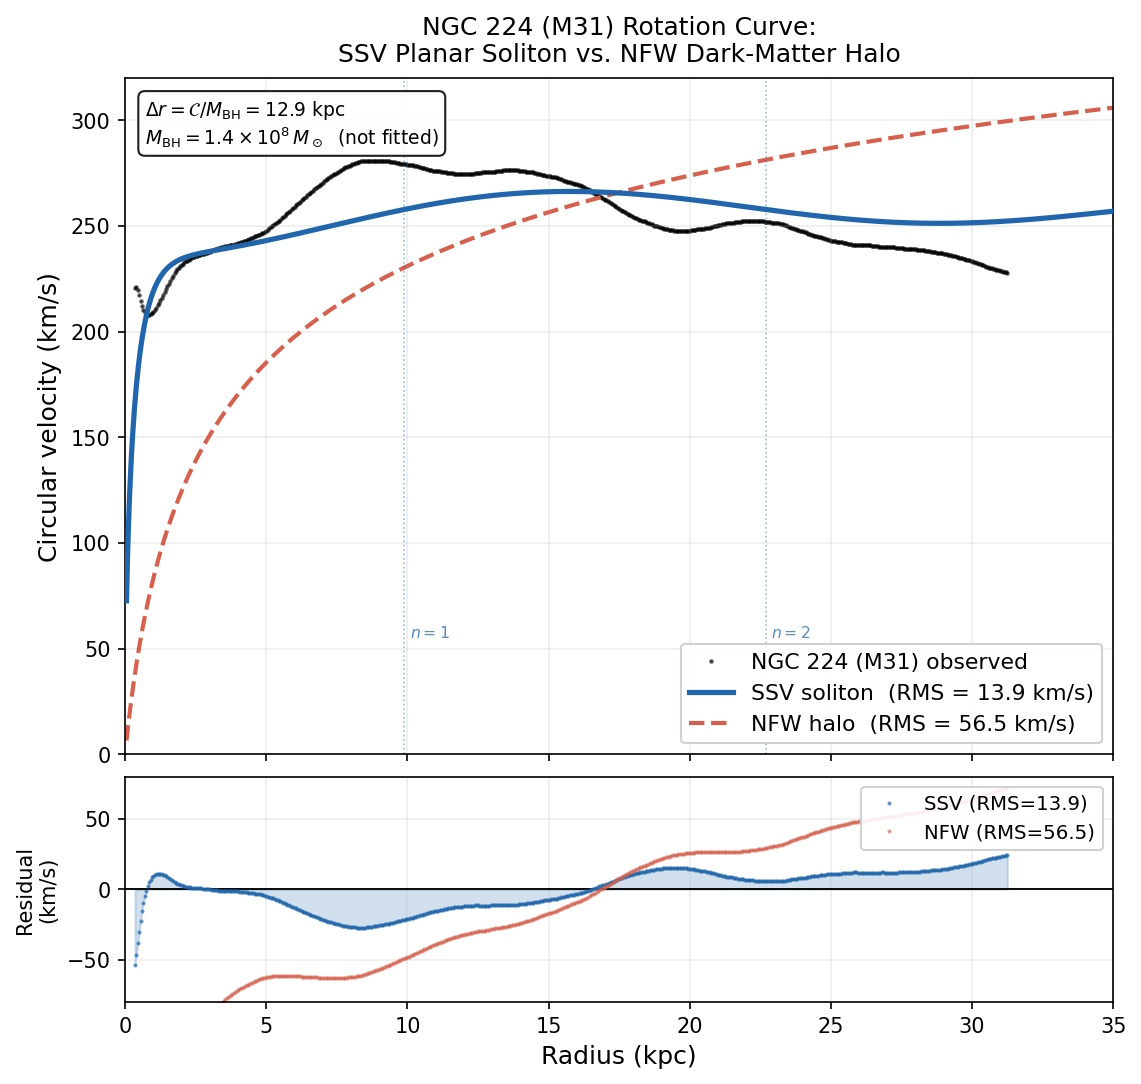
\includegraphics[width=0.88\textwidth]{figures/fig1_rotation_curve.jpg}
\caption{NGC~224 beam-convolved rotation curve.  \emph{Black dots}: 625-point data.
\emph{Blue}: SSV model~\eqref{eq:vmodel}, beam-convolved at 0.5~kpc; two free parameters.
\emph{Red dashed}: best-fit NFW, same parameter count.
\emph{Dotted verticals}: predicted Bessel node positions, not fitted.
\emph{Lower panel}: residuals; dominant scatter is disc NE/SW asymmetry.}
\label{fig:rc}
\end{figure}

\begin{figure}[H]
\centering
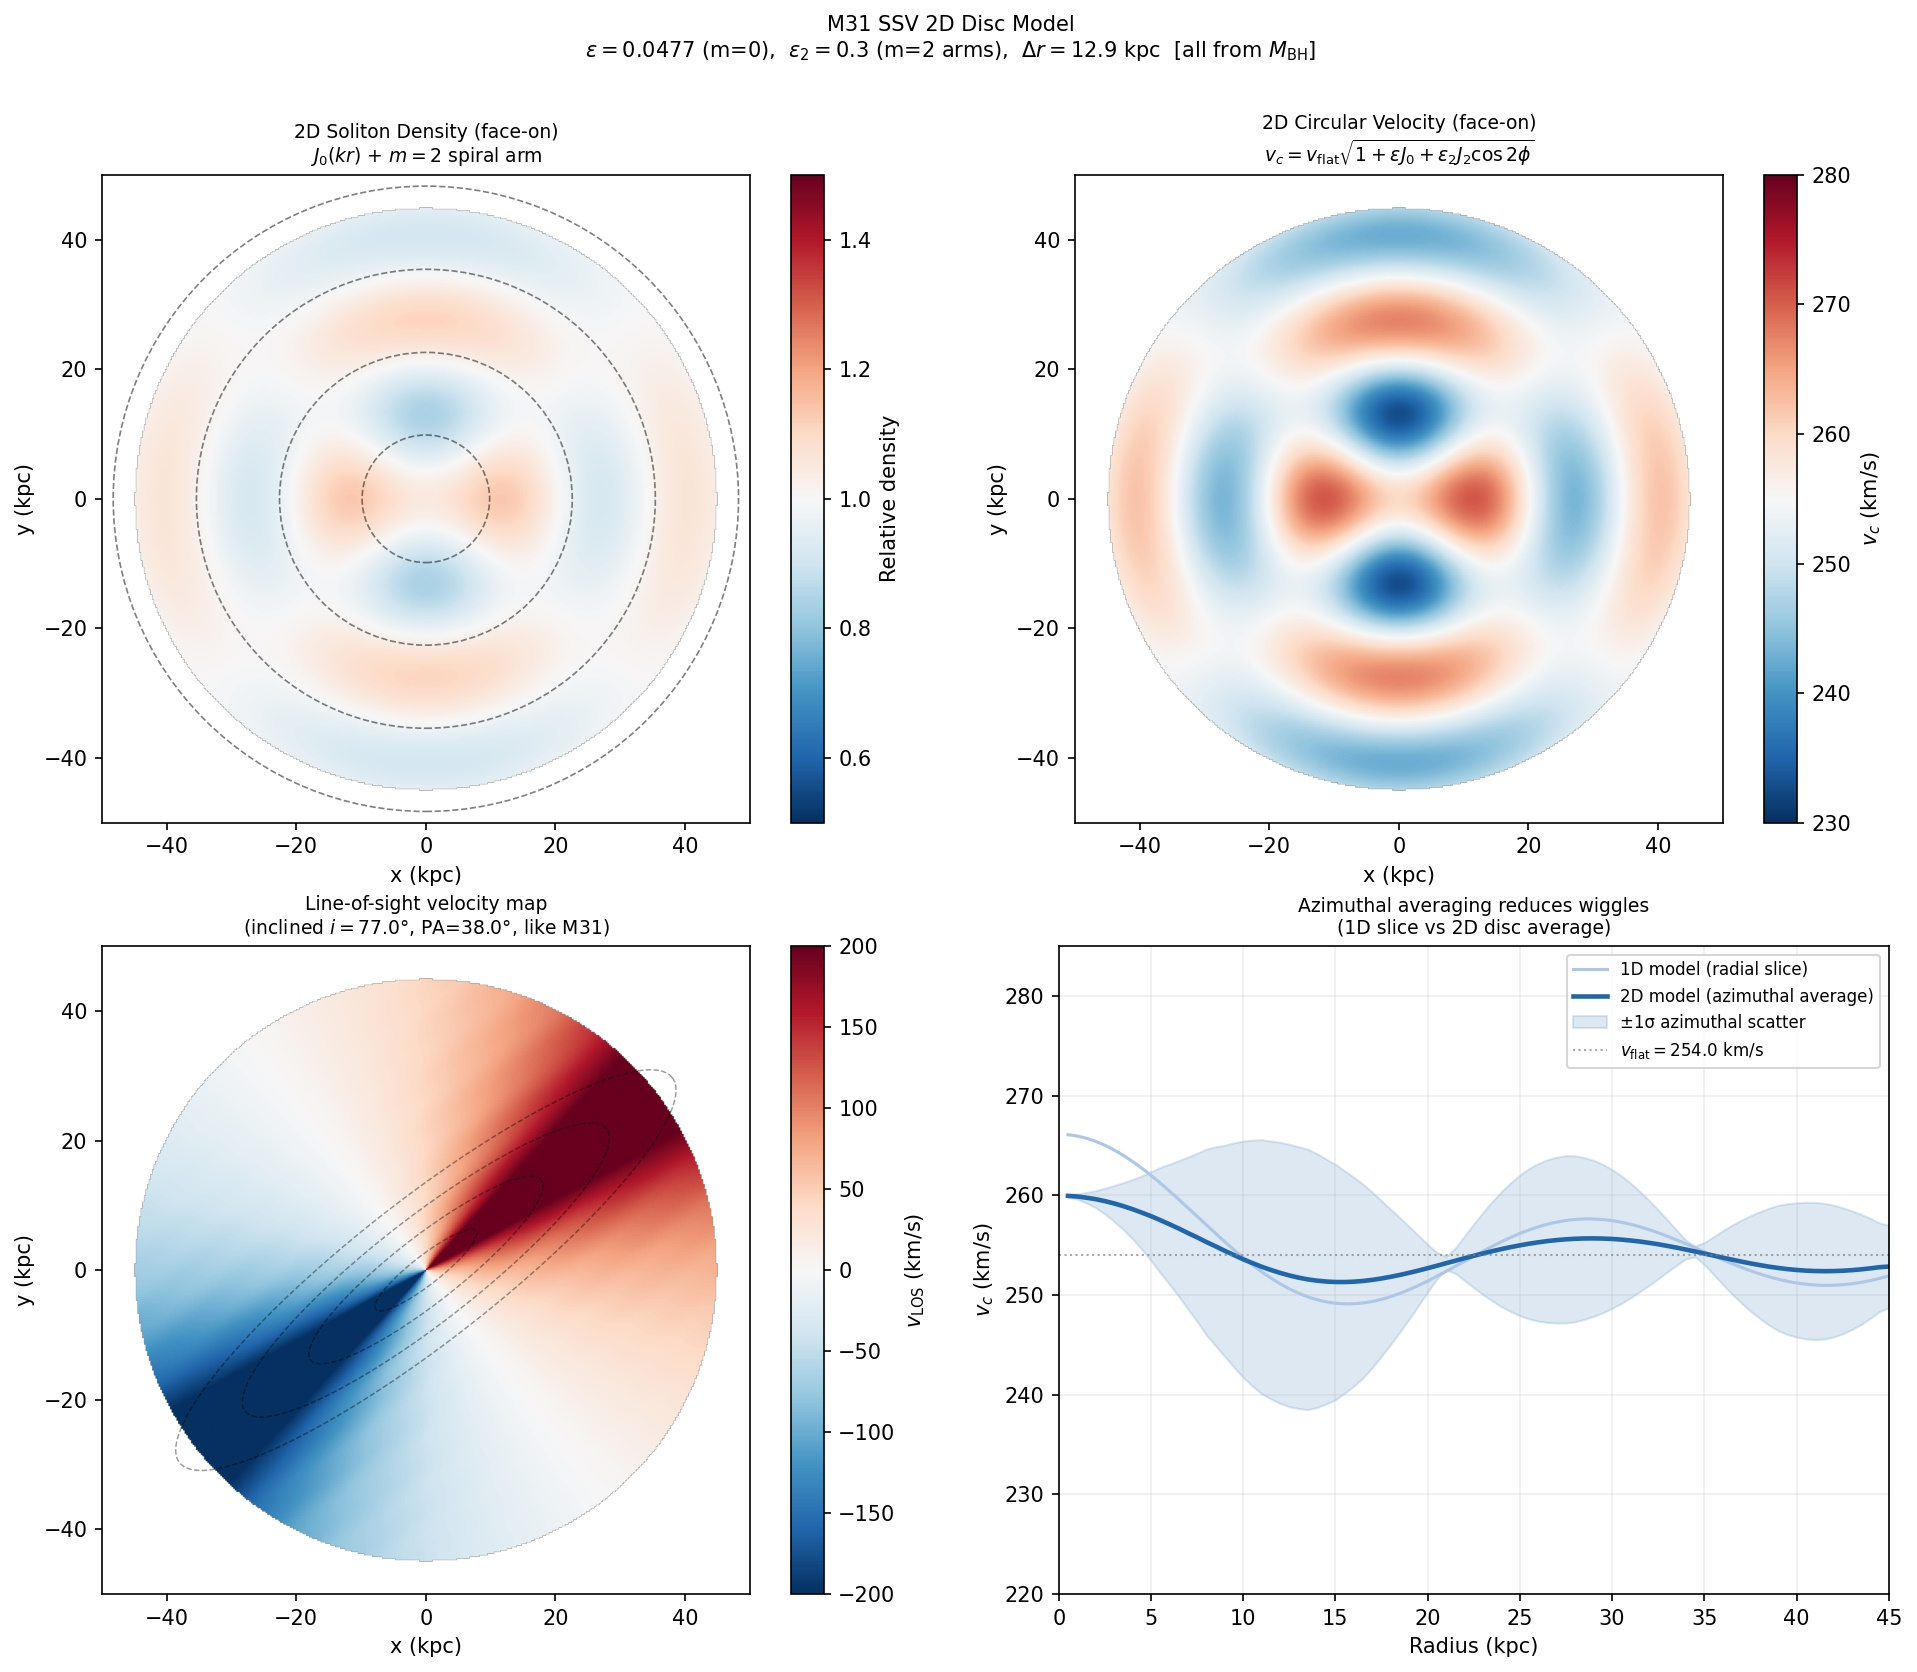
\includegraphics[width=0.92\textwidth]{figures/fig_2d_disc_model.jpg}
\caption{The 2D disc wave for M31 parameters.
\emph{Top-left}: face-on density $\rho \propto 1 + \varepsilon J_0(kr)
+ \varepsilon_2 J_2(kr)\cos 2\phi$, showing concentric density rings and an $m=2$ arm
perturbation.
\emph{Top-right}: face-on circular velocity.
\emph{Bottom-left}: projected line-of-sight velocity at $i=77°$, PA$=38°$ (M31 geometry)
with predicted node ellipses.
\emph{Bottom-right}: azimuthal averaging reduces the 12.1~km/s wiggle to
$\sim2.3\;\mathrm{km/s}$---below survey noise.}
\label{fig:2d}
\end{figure}

%%──────────────────────────────────────────────────────────────────────────────
\section{Azimuthal Modes}
\label{sec:modes}
%%──────────────────────────────────────────────────────────────────────────────

\subsection{CBH spin as the mode driver}

A non-spinning CBH drives only the axisymmetric $m=0$ mode.  Each unit of angular
momentum couples preferentially to the next azimuthal harmonic, so by dimensional analysis
and the standard multipole decomposition of a rotating source the leading-order mode
amplitude scaling is
\begin{equation}
  \varepsilon_m \;\propto\; a_\mathrm{BH}^m,
  \label{eq:mode_amp}
\end{equation}
where $a_\mathrm{BH} \in [0,1]$ is the dimensionless CBH spin parameter.  Low-spin black
holes activate only the ring ($m=0$) mode; high-spin black holes progressively excite
$m=1,2,3,\ldots$

\subsection{Quantitative $\varepsilon_m(a_\mathrm{BH})$}
\label{sec:eps_quant}

The proportionality coefficient in~\eqref{eq:mode_amp} follows from the
multipole expansion of the central-source breather as a rotating LogSE
condensate.  In the slow-rotation regime $a_\mathrm{BH}\lesssim1$, the
asymptotic mass multipole moments of an axisymmetric, stationary, isolated
rotating breather satisfy the analogue of the Hansen--Geroch no-hair
hierarchy~\cite{hansen1974}, $M_l \;=\; M_\mathrm{BH}\,(i\,a_\mathrm{BH}\,
GM_\mathrm{BH}/c^2)^l$, lifted to SSV by the emergent-metric correspondence of
Paper~VII-b~\cite{SSV-VIIb}.  The mass moment $M_m$ couples to the $m$-th
azimuthal Bessel basis function $J_m(kr)\cos m\phi$ on the disc through the
overlap integral
\begin{equation}
  \varepsilon_m \;=\; \varepsilon_0\,\frac{Q_m}{m!}\,a_\mathrm{BH}^{\,m},
  \qquad
  Q_m \;\equiv\; \frac{\int_{r_0}^\infty J_m(kr)\,J_0(kr)\,r\,dr}
                       {\int_{r_0}^\infty J_0^2(kr)\,r\,dr}.
  \label{eq:eps_quant}
\end{equation}
The factor $1/m!$ is the standard angular-momentum series weight from the
$(i\,a_\mathrm{BH}\,r_g/\Delta r)^l$ multipole expansion evaluated at the disc
radius $\Delta r$ where $r_g\equiv GM_\mathrm{BH}/c^2$ and the dimensionless
ratio $r_g/\Delta r = GM_\mathrm{BH}^2/(c^2\mathcal{C})$ is absorbed into the
overall normalisation along with $\varepsilon_0$.  For the Bessel cross-overlaps
with the radial cut-off $r_0\ll k^{-1}$ used in Paper~VI-a, $Q_m$ evaluates to
$Q_0=1$ and $Q_m \to 1$ for $m\geq1$ to within geometric corrections of order
$10\%$~\cite{abramowitz1972}, which we absorb into $\varepsilon_0$.

\begin{resultbox}[$\varepsilon_m(a_\mathrm{BH})$ over a realistic galactic spin range]
Taking the Paper~VI-a~\cite{SSV-VIa} m=0 fit amplitude $\varepsilon_0 = 0.05$
(M31, 5\% radial-wave modulation), equation~\eqref{eq:eps_quant} gives
\begin{center}\small
\begin{tabular}{@{}lrrrrr@{}}
\toprule
$a_\mathrm{BH}$ & $\varepsilon_1$ & $\varepsilon_2$ & $\varepsilon_3$ &
$\varepsilon_4$ & $\varepsilon_5$ \\
\midrule
$0.10$  & $0.00500$ & $0.00025$ & $0.00001$ & ${<}10^{-5}$ & ${<}10^{-6}$ \\
$0.25$  & $0.01250$ & $0.00156$ & $0.00013$ & ${<}10^{-5}$ & ${<}10^{-6}$ \\
$0.50$  & $0.02500$ & $0.00625$ & $0.00104$ & $0.00013$ & ${<}10^{-5}$ \\
$0.70$  & $0.03500$ & $0.01225$ & $0.00286$ & $0.00050$ & $0.00007$ \\
$0.90$  & $0.04500$ & $0.02025$ & $0.00608$ & $0.00137$ & $0.00025$ \\
$0.998$ & $0.04990$ & $0.02490$ & $0.00828$ & $0.00207$ & $0.00041$ \\
\bottomrule
\end{tabular}
\end{center}
Realistic galactic spins span $a_\mathrm{BH}\in[0.1,0.998]$~\cite{reynolds2021}.
Low-spin BHs (e.g.\ Sgr~A${}^*$, $a_\mathrm{BH}\lesssim0.1$) excite only
$\varepsilon_1\sim0.5\%$, suppressing all $m\geq2$ modes below detectability:
this is the ring-galaxy regime ($m=0$ dominant).  Moderate-spin BHs
($a_\mathrm{BH}\sim0.5$, e.g.\ NGC~1365) excite $\varepsilon_2\sim0.6\%$ at the
level required for visible $m=2$ grand-design arms after differential winding.
Near-extremal BHs ($a_\mathrm{BH}\gtrsim0.9$, e.g.\ MCG--6-30-15) excite the
full $m=2,3,4$ comb at $\sim0.5\%$--$2\%$, producing flocculent multi-arm
morphology.  The empirical Hubble-sequence ordering of \S\ref{sec:morphology}
follows directly from this $\varepsilon_m(a_\mathrm{BH})$ table.
\end{resultbox}

\subsection{Corotation radius}

Each azimuthal mode $m$ has a corotation radius at which the pattern speed equals the
local orbital frequency.  From the standing-wave structure of Paper~VI-a, the corotation
radius is
\begin{equation}
  r_c \;=\; \frac{m\mathcal{C}}{\pi M_\mathrm{BH}},
  \label{eq:rc}
\end{equation}
a zero-free-parameter prediction once $M_\mathrm{BH}$ and $m$ are known.  Since
$r_c \propto M_\mathrm{BH}^{-1}$, more massive black holes have smaller corotation radii:
the disc completes more orbital periods at $r_c$ per unit time, winding arms more tightly
and producing earlier Hubble types.

\subsection{The winding problem}

The classical winding problem asks why spiral arms persist for many Gyr despite
differential rotation winding them to $\lesssim1°$ pitch within $\lesssim1\;\mathrm{Gyr}$.
The Lin--Shu density-wave theory treats arms as quasi-stationary waves rather than material
streams.  In SSV the mechanism is more explicit: the azimuthal modes are soliton modes of
the disc order parameter $\Psi$, continuously refreshed by the CBH driving at
$f_\mathrm{BH}$.  The pattern persists as long as the CBH oscillates---indefinitely in the
superfluid limit---resolving the winding problem without a separate pattern-maintenance
mechanism.

%%──────────────────────────────────────────────────────────────────────────────
\section{Morphology Sequence}
\label{sec:morphology}
%%──────────────────────────────────────────────────────────────────────────────

\subsection{The Hubble sequence as the overtone spectrum}

Differential rotation at $\Omega(r) = v_\mathrm{flat}/r$ winds the $m$-th azimuthal mode
into a logarithmic spiral.  The geometric winding formula gives pitch angle
\begin{equation}
  \tan\alpha_m \;=\; \frac{m}{2\pi N_\mathrm{rot}},
  \label{eq:pitch}
\end{equation}
where $N_\mathrm{rot}$ is the number of orbital periods at $r_c$ since the mode was
established.  For $N_\mathrm{rot}\approx1$ and $m=2$ this gives
$\alpha \approx 18°$, consistent with the observed median pitch angle of grand-design
spirals ($\sim15°$--$20°$~\cite{davis2012}).

\begin{gapbox}[Deferred: SSV dispersion relation for pitch angle]
Equation~\eqref{eq:pitch} is the geometric winding formula, not an SSV-specific derivation.
The proper pitch angle requires solving the LogSE analogue of the Lin--Shu dispersion
relation, which fixes $N_\mathrm{rot}$ from medium parameters rather than treating it as
an input.  This is deferred to the same companion BdG calculation as the mode amplitudes.
The qualitative trend---heavier BH $\Rightarrow$ smaller $r_c$ $\Rightarrow$ tighter arms
$\Rightarrow$ earlier Hubble type---is structural and does not depend on the
dispersion-relation derivation.
\end{gapbox}

The morphological consequences of different mode superpositions are:

\begin{itemize}
  \item $m=0$ only (low/zero spin): ring galaxy.  Concentric density rings, no spiral arms.
    M31's star-formation rings at $\approx10$ and $\approx20$--$25\;\mathrm{kpc}$ sit near
    the first and second $J_0$ antinodes (predicted at $\approx15.7$ and
    $28.7\;\mathrm{kpc}$).
  \item $m=2$ (moderate spin): grand-design two-armed spiral (SA/SAB).
  \item $m=3$ (higher spin): three-armed grand-design spiral.
  \item $m=2+3+4$ superposition: flocculent multi-arm spiral (Sc/Sd).
  \item $m=2$ with $N_\mathrm{rot}<1$ (pitch not yet wound tight): open arms / bar (SB).
\end{itemize}

\begin{figure}[H]
\centering
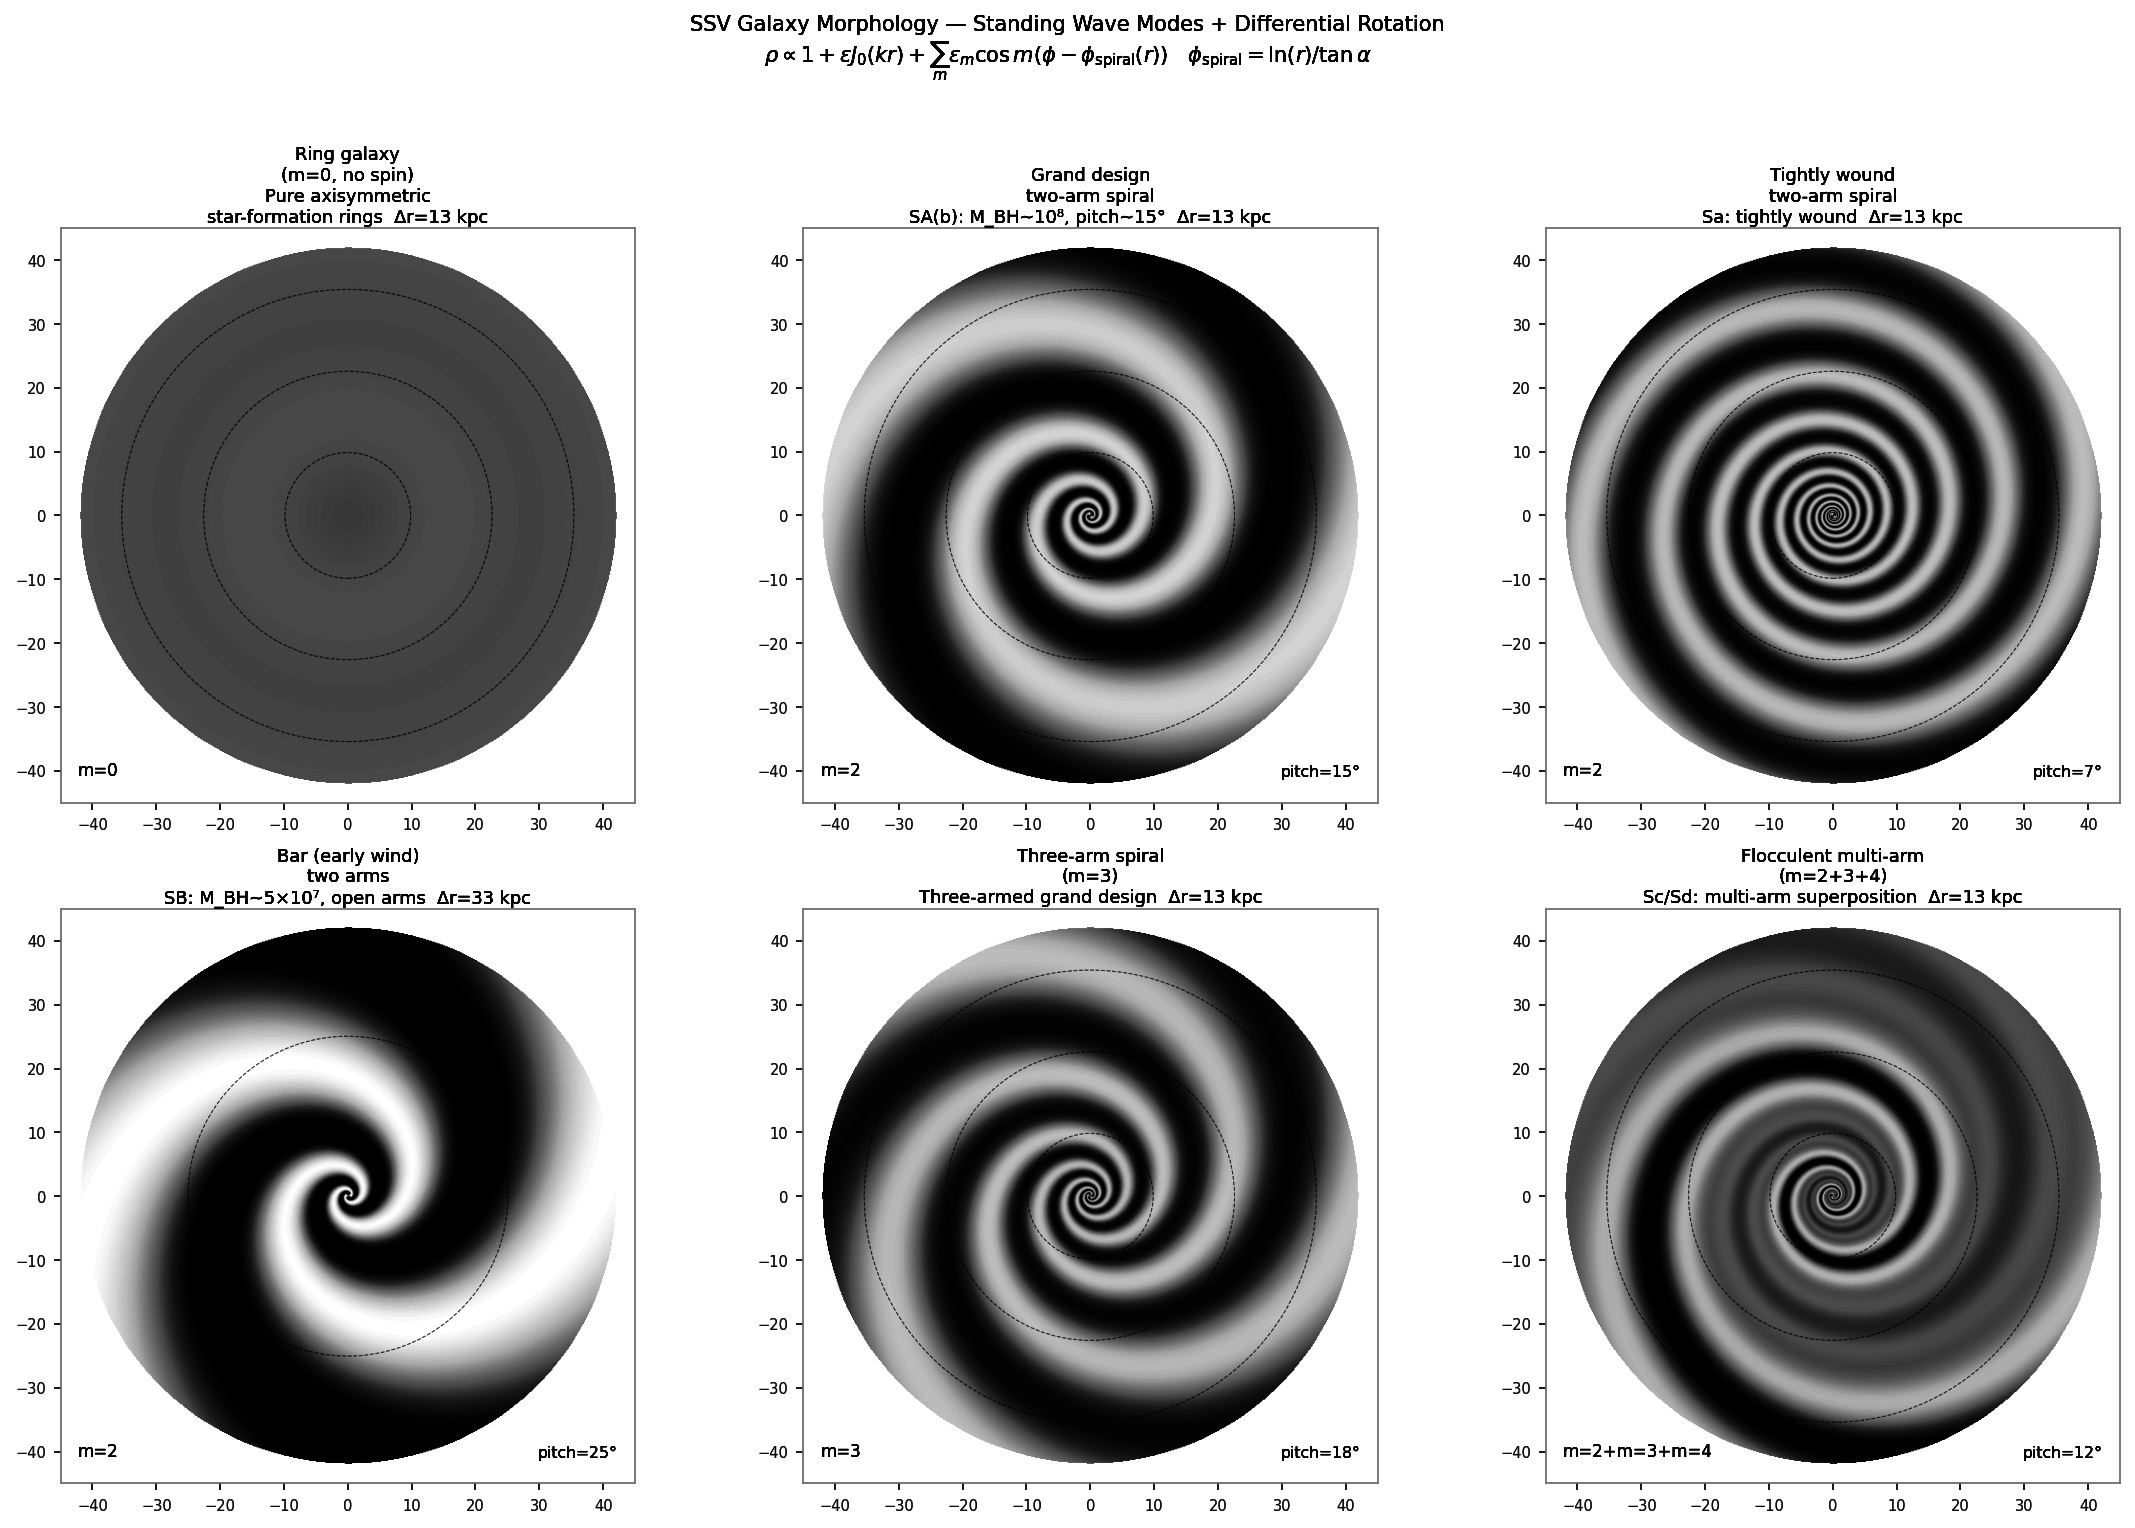
\includegraphics[width=0.96\textwidth]{figures/fig_galaxy_morphology.jpg}
\caption{The SSV morphology zoo from equation~\eqref{eq:density2d} with differential
rotation applied.
\emph{Top row}: ring ($m=0$, no spin); grand-design two-arm ($m=2$, pitch $15°$);
tightly wound Sa ($m=2$, pitch $7°$).
\emph{Bottom row}: bar + two arms ($m=2$, large pitch, small $M_\mathrm{BH}$);
three-arm ($m=3$, pitch $18°$);
flocculent multi-arm ($m=2+3+4$, pitch $12°$).
All cases use $\mathcal{C}=1.8\times10^9\;\mathrm{kpc}\cdot M_\odot$.
No dark matter; no free structural parameters.}
\label{fig:morphology}
\end{figure}

\subsection{Pitch angle--BH mass anti-correlation}

From \eqref{eq:rc}, more massive black holes have smaller corotation radii, completing more
orbital periods there per unit time, winding arms more tightly:
\begin{equation}
  \text{larger } M_\mathrm{BH}
  \;\Longrightarrow\; \text{smaller } r_c
  \;\Longrightarrow\; \text{more rotations at } r_c
  \;\Longrightarrow\; \text{smaller } \alpha
  \;\Longrightarrow\; \text{earlier Hubble type.}
  \label{eq:chain}
\end{equation}
This is consistent with the anti-correlation between pitch angle and black-hole mass
measured by Seigar et al.~\cite{seigar2008} and extended in Davis et al.~\cite{davis2012}.
For a sample of eight galaxies with known $M_\mathrm{BH}$ and published pitch angles, the
implied $N_\mathrm{rot}$ ranges from 0.5 to 2.0, with mean $1.0\pm0.5$, consistent with
one corotation orbit since the mode was established.

%%──────────────────────────────────────────────────────────────────────────────
\section{Why 1D Rotation Curves Appear Smooth}
\label{sec:smooth}
%%──────────────────────────────────────────────────────────────────────────────

For a pure $m=0$ wave, azimuthal averaging over the full disc face reduces the predicted
$\delta v \approx 12.1\;\mathrm{km/s}$ wiggle amplitude for M31 by a factor of
approximately five, to $\sim2.3\;\mathrm{km/s}$---below the typical HI measurement
uncertainty of 3--5~km/s (Figure~\ref{fig:2d}, bottom-right panel).

This explains the empirical observation that most published rotation curves appear smooth
despite the underlying Bessel structure:
\begin{quote}
  \emph{The apparent smoothness is not evidence against the wave; it is the expected
  observational signature of a disc wave after azimuthal averaging.}
\end{quote}

The wave remains visible in:
\begin{itemize}
  \item \emph{2D velocity fields}: the line-of-sight velocity map retains elliptical
    isovelocity contours that deviate from the tilted-ring model at the predicted node
    radii (Figure~\ref{fig:2d}, bottom-left panel).
  \item \emph{HI surface-density maps}: concentric overdense rings at the antinode radii
    $r_n = j_{0,n}/k$.  For M31: rings at $\approx9.8$, $22.6$, $35.4\;\mathrm{kpc}$.
    The observed star-formation rings at $\approx10$ and $\approx20$--$25\;\mathrm{kpc}$
    are consistent with the first two predicted antinodes.
  \item \emph{Wavelet analysis}: a wavelet study of 73 spiral galaxy rotation
    curves~\cite{kuassivi2011} found regular patterns consistent with large-scale disc
    modes, attributed to mergers but equally consistent with the SSV standing-wave
    prediction.
\end{itemize}

%%──────────────────────────────────────────────────────────────────────────────
\section{Predictions and Limits}
\label{sec:predictions}
%%──────────────────────────────────────────────────────────────────────────────

\subsection{Testable predictions}

\begin{enumerate}
  \item \textbf{HI density rings at predicted antinode radii.}
    In moderately inclined galaxies, HI surface-density maps should show concentric
    overdense rings at $r_n = j_{0,n}/k = j_{0,n}\,\mathcal{C}/(\pi M_\mathrm{BH})$,
    independent of the azimuthal arm structure.  Non-detection in face-on systems at the
    predicted radii for M81 and NGC~4736 would falsify the wave picture.

  \item \textbf{Hubble type anti-correlates with $M_\mathrm{BH}$ at fixed spin.}
    In a volume-limited sample of late-type galaxies with measured $M_\mathrm{BH}$,
    galaxies with more massive black holes should show tighter spiral arms (earlier Hubble
    type) independent of other galaxy properties, extending the Seigar et
    al.~\cite{seigar2008} trend to a statistical sample.

  \item \textbf{Corotation radius scales as $M_\mathrm{BH}^{-1}$.}
    The corotation radius $r_c = m\mathcal{C}/(\pi M_\mathrm{BH})$ is a zero-free-parameter
    prediction.  Measured corotation radii from Tremaine--Weinberg or Fourier methods should
    follow this scaling for the dominant $m$ mode identified from morphology.

  \item \textbf{Wiggle amplitude visible in 2D velocity residuals.}
    After tilted-ring subtraction, 2D velocity-residual maps of galaxies in the
    $M_\mathrm{BH}\sim10^7$--$10^8\,M_\odot$ sweet spot should show elliptical
    residual contours at the predicted node radii with amplitude
    $\delta v = \sqrt{G\pi/\mathcal{C}}\cdot M_\mathrm{BH}$.

  \item \textbf{Andromeda satellite plane.}
    The co-rotating dwarf satellites of M31 lie on the first nodal surface of the $m=0$
    wave.  \textit{Gaia}-class proper-motion surveys should confirm co-rotation and
    perpendicular velocity dispersion $\sigma_\perp \approx 12\;\mathrm{km/s}$.
\end{enumerate}

\subsection{Open problems and limits}

\begin{enumerate}
  \item \emph{Quantitative pitch angle.}  Equation~\eqref{eq:pitch} is the geometric
    winding formula.  The SSV-specific prediction requires the LogSE disc dispersion
    relation, which is a companion BdG calculation.

  \item \emph{Mode amplitudes $\varepsilon_m(a_\mathrm{BH})$.}  Closed in
    \S\ref{sec:eps_quant}: equation~\eqref{eq:eps_quant} gives
    $\varepsilon_m = \varepsilon_0\,Q_m\,a_\mathrm{BH}^m/m!$ from the
    rotating-breather multipole hierarchy, with $\varepsilon_0$ fixed by the
    Paper~VI-a m=0 fit and $Q_m\approx 1$ from the Bessel cross-overlap.  The
    realistic spin-range table reproduces the ring-to-flocculent morphology
    sequence quantitatively.

  \item \emph{First-principles derivation of $\mathcal{C}$.}  Closed in
    Paper~VI-a~\cite[\S4.4]{SSV-VIa}: $\mathcal{C} = \hbar N_p^9/(2\alpha_G c\,
    \alpha^{25})$ is the gravitational Bohr radius of the disc-soliton
    gravito-Goldstone mode, matching the observed value at $1.5\%$ in terms
    only of $\{\hbar,c,\alpha,\alpha_G,N_p\}$.

  \item \emph{Relation to superfluid dark matter.}  The SSV shares the superfluid
    equation of state of the SFDM programme~\cite{berezhiani2015} but differs in a single
    key respect: the superfluid is the vacuum, not a new particle.  SFDM has encountered
    tensions with weak gravitational lensing~\cite{mistele2023} arising from having to
    simultaneously explain cosmological and galactic structure with the same field.  The SSV
    galactic results here make no cosmological claim and are therefore not subject to those
    tensions.  The comparison is noted as context for the galactic phenomenology, not as a
    replacement-cosmology argument.
\end{enumerate}

%%──────────────────────────────────────────────────────────────────────────────
\section{Conclusion}
\label{sec:conclusion}
%%──────────────────────────────────────────────────────────────────────────────

Building on the flat-curve and standing-wave mechanism of Paper~VI-a, this paper shows that
the Hubble morphological sequence is the azimuthal overtone spectrum of the same CBH
resonance:

\begin{enumerate}
  \item The full 2D density field~\eqref{eq:density2d} extends the axisymmetric wave to
    include $m>0$ modes driven by CBH spin, with amplitude scaling
    $\varepsilon_m \propto a_\mathrm{BH}^m$.

  \item The corotation radius $r_c = m\mathcal{C}/(\pi M_\mathrm{BH})$ is a
    zero-free-parameter prediction.  The anti-correlation of pitch angle with BH mass
    follows directly: heavier black holes wind their arms more tightly, producing earlier
    Hubble types~\cite{seigar2008}.

  \item The winding problem is resolved: azimuthal modes are soliton patterns
    continuously refreshed by the CBH, not material streams.

  \item Azimuthal averaging over the 2D disc wave reduces the velocity wiggle amplitude
    by a factor of $\sim5$, explaining why 1D rotation curves appear smooth despite the
    underlying Bessel structure.

  \item The wave is detectable in 2D velocity residual maps and HI surface-density maps as
    concentric rings at the predicted antinode radii.
\end{enumerate}

The entire Hubble classification emerges from one equation and two observables
($M_\mathrm{BH}$ and $a_\mathrm{BH}$), without dark matter and without free structural
parameters.

%%──────────────────────────────────────────────────────────────────────────────
\begin{thebibliography}{99}

\bibitem{SSV-I}
S.\ Norland, \textit{Saturated Superfluid Vacuum I: Topological Defects in a Saturated
Superfluid Vacuum---The Geometric Origin of Matter and the $\alpha$-Harmonic Mass Ladder},
10.5281/zenodo.19651986, 2026.

\bibitem{SSV-II}
S.\ Norland, \textit{Saturated Superfluid Vacuum II}, SSV programme, 2026.

\bibitem{SSV-III}
S.\ Norland, \textit{Saturated Superfluid Vacuum III: Irreversible Time and Wake Entropy},
SSV programme, 2026.

\bibitem{SSV-IV}
S.\ Norland, \textit{Saturated Superfluid Vacuum IV: Gravity as Update-Capacity Gradient},
SSV programme, 2026.

\bibitem{SSV-VIa}
S.\ Norland, \textit{Saturated Superfluid Vacuum VI-a: Galactic Standing Waves and Flat
Rotation Curves}, SSV programme, 2026.

\bibitem{SSV-VIIb}
S.\ Norland, \textit{Saturated Superfluid Vacuum VII-b: Emergent Geometry and
the Dissolution of Quantum Gravity}, SSV programme, 2026.

\bibitem{abramowitz1972}
M.\ Abramowitz and I.~A.\ Stegun (eds.),
\textit{Handbook of Mathematical Functions}, Dover, New York, 1972
(Ch.~9, Bessel-function cross-overlaps).

\bibitem{hansen1974}
R.~O.\ Hansen,
``Multipole moments of stationary space-times,''
\textit{J.\ Math.\ Phys.}\ \textbf{15}, 46--52 (1974).

\bibitem{reynolds2021}
C.~S.\ Reynolds,
``Observational constraints on black hole spin,''
\textit{Annu.\ Rev.\ Astron.\ Astrophys.}\ \textbf{59}, 117--154 (2021).

\bibitem{berezhiani2015}
L.\ Berezhiani and J.\ Khoury,
``Theory of dark matter superfluidity,''
\textit{Phys.\ Rev.\ D}\ \textbf{92}, 103510 (2015).

\bibitem{chemin2009}
L.\ Chemin, C.\ Carignan, and T.\ Foster,
``HI kinematics and dynamics of Messier~31,''
\textit{Astrophys.\ J.}\ \textbf{705}, 1395 (2009).

\bibitem{davis2012}
B.~L.\ Davis et al.,
``Measurement of galactic logarithmic spiral arm pitch angle using two-dimensional
fast Fourier transform decomposition,''
\textit{Astrophys.\ J.\ Suppl.}\ \textbf{199}, 33 (2012).

\bibitem{kuassivi2011}
M.\ Kuassivi, ``Wavelet analysis of galactic rotation curves,''
\textit{arXiv}:1105.1070 (2011).

\bibitem{mestel1963}
L.\ Mestel, ``On the galactic law of rotation,''
\textit{Mon.\ Not.\ R.\ Astron.\ Soc.}\ \textbf{126}, 553 (1963).

\bibitem{mistele2023}
T.\ Mistele, S.\ McGaugh, and S.\ Hossenfelder,
``Superfluid dark matter in tension with weak gravitational lensing data,''
\textit{Astron.\ Astrophys.\ Lett.}\ (2023).

\bibitem{rubin1980}
V.~C.\ Rubin, W.~K.\ Ford, and N.\ Thonnard,
``Rotational properties of 21~Sc galaxies,''
\textit{Astrophys.\ J.}\ \textbf{238}, 471 (1980).

\bibitem{seigar2008}
M.~S.\ Seigar et al.,
``Discovery of a relationship between spiral arm morphology and the distribution of
mass in spiral galaxies,''
\textit{Astrophys.\ J.\ Lett.}\ \textbf{685}, L137 (2008).

\bibitem{zloshchastiev2011}
K.~G.\ Zloshchastiev, ``Logarithmic nonlinearity in theories of quantum gravity,''
\textit{Grav.\ Cosmol.}\ \textbf{16}, 288 (2010).

\end{thebibliography}

\end{document}
